\documentclass[10pt,twocolumn]{article}
\usepackage[utf8]{inputenc}
\usepackage[english]{babel}
\usepackage{amsmath,amssymb,amsfonts}
\usepackage{graphicx}
\usepackage{booktabs}
\usepackage{algorithm}
\usepackage{algorithmic}
\usepackage{hyperref}
\usepackage[letterpaper,margin=0.75in]{geometry}
\usepackage{cite}

\title{FedForget: Federated Unlearning via Dual-Teacher Knowledge Distillation}

\author{
Anonymous Authors\\
Anonymous Institution\\
\texttt{anonymous@example.com}
}

\date{}

\begin{document}

\maketitle

\begin{abstract}
Federated learning enables collaborative model training without centralizing data, but the ``Right to be Forgotten'' requires efficient mechanisms to remove specific clients' data contributions. Existing federated unlearning methods face a fundamental limitation: single-teacher knowledge distillation uses a contaminated teacher model that contains knowledge from the forgetting client, leading to incomplete unlearning and privacy leakage. We propose \textbf{FedForget}, a novel federated unlearning framework that addresses this challenge through \textbf{dual-teacher knowledge distillation} combined with server-side dynamic weight adjustment. Our key insight is that effective unlearning requires two complementary teachers: a global teacher preserving overall knowledge structure, and a local teacher providing ``clean'' reference without the forgetting client's influence. Through comprehensive experiments on CIFAR-10 with 5 and 10 clients, we demonstrate that FedForget achieves superior multi-objective balance: 20.01$\pm$1.92\% forgetting rate, 96.57$\pm$1.21\% retention, and near-ideal privacy protection (ASR=52.91$\pm$2.32\%, closest to ideal 50\%). Notably, FedForget exhibits counter-intuitive scalability---performance improves with 10 clients (+2.09\% retention, -2.68\% ASR improvement), demonstrating strong applicability to large-scale federated systems. Our ablation study validates that dual-teacher distillation contributes +11.54\% retention compared to single-teacher approaches, while achieving 1.53-1.75$\times$ speedup over complete retraining.
\end{abstract}

\textbf{Keywords:} Federated Learning, Machine Unlearning, Knowledge Distillation, Privacy Protection, GDPR Compliance

\section{Introduction}

\subsection{Motivation and Background}

Federated Learning (FL) \cite{mcmahan2017communication} has emerged as a promising paradigm for collaborative machine learning, enabling multiple clients to jointly train a shared global model without exposing their raw data. By keeping data decentralized and performing computation on local devices, FL addresses critical privacy concerns in domains such as healthcare \cite{rieke2020future}, finance \cite{yang2019federated}, and mobile applications \cite{hard2018federated,kairouz2021advances,li2020federated}.

However, the right to data deletion---enshrined in privacy regulations such as GDPR's ``Right to be Forgotten'' \cite{gdpr2018} and CCPA \cite{ccpa2020}---poses a significant challenge for federated learning systems. When a client requests to remove their data contribution from a trained model, the straightforward solution is to \textbf{retrain the model from scratch} excluding that client's data. Unfortunately, retraining is prohibitively expensive in large-scale federated settings, where training may involve hundreds or thousands of clients over days or weeks \cite{yang2019federated,bonawitz2019towards}.

This challenge has motivated the development of \textbf{Machine Unlearning} \cite{cao2015towards,bourtoule2021machine}---techniques that efficiently remove the influence of specific training data from a learned model without full retraining. While unlearning has been extensively studied in centralized settings \cite{golatkar2020eternal,tarun2021fast,guo2020certified,thudi2022necessity}, \textbf{Federated Unlearning} introduces unique challenges:

\begin{enumerate}
\item \textbf{Data Heterogeneity}: Clients have Non-IID (non-identically distributed) data \cite{zhao2018federated,hsu2019measuring}, making it difficult to remove specific client contributions while preserving global model utility
\item \textbf{Privacy Constraints}: The server cannot access raw client data, limiting the applicability of centralized unlearning techniques
\item \textbf{Catastrophic Forgetting}: Naive unlearning approaches (e.g., gradient ascent on forgetting data) can cause the model to forget not only the target data but also unrelated knowledge
\item \textbf{Multi-Objective Trade-off}: Balancing unlearning effectiveness, model utility preservation, privacy protection, and computational efficiency simultaneously
\end{enumerate}

\subsection{Limitations of Existing Approaches}

Recent federated unlearning methods \cite{liu2021federaser,wu2023federated,ferrari2024efficient,gao2022verifi} have made important progress, but face key limitations:

\textbf{Calibration-Based Methods} \cite{liu2021federaser,gao2022verifi} calibrate the global model using remaining clients' data. However, they often achieve \textbf{limited unlearning effectiveness}, as they do not actively remove the forgetting client's influence.

\textbf{Knowledge Distillation Methods} \cite{wu2023federated} use the pre-trained global model as a teacher to guide unlearning. However, \textbf{single-teacher distillation} has a fundamental flaw: the teacher model itself contains knowledge from the forgetting client, leading to incomplete unlearning and privacy leakage.

\textbf{Feature-Based Methods} \cite{ferrari2024efficient} focus on removing feature-level influence via maximum mean discrepancy. While effective for specific feature-based attacks, they may not provide comprehensive privacy guarantees against diverse inference attacks.

\textbf{Common Weakness}: None of these methods achieve optimal balance across all four objectives---effectiveness, utility, privacy, and efficiency---simultaneously. More importantly, existing single-teacher distillation approaches fail to provide a ``clean'' reference model, limiting their unlearning completeness.

\subsection{Our Approach: FedForget}

We propose \textbf{FedForget}, a novel federated unlearning framework that addresses these limitations through \textbf{dual-teacher knowledge distillation} combined with \textbf{server-side dynamic weight adjustment}. Our key insight is:

\begin{quote}
\textit{Dual-Teacher Synergy: Effective federated unlearning requires two complementary teachers---one preserving overall model structure (global teacher), and one providing ``clean'' reference without the forgetting client's influence (local teacher).}
\end{quote}

\textbf{Core Innovations:}

\begin{enumerate}
\item \textbf{Dual-Teacher Knowledge Distillation}: Teacher A (Global Teacher) preserves overall knowledge structure using the pre-trained global model. Teacher B (Local Teacher) provides clean reference using a model trained only on remaining clients' data. This synergistic effect prevents catastrophic forgetting while enabling precise unlearning, achieving +11.54\% retention compared to single-teacher distillation.

\item \textbf{Server-Side Dynamic Weight Adjustment}: Exponentially decay the forgetting client's aggregation weight over unlearning rounds ($w_f^{(t)} = w_f^{(0)} \cdot \exp(-\lambda_{\text{forget}} \cdot t)$), creating a smooth transition from pre-trained model to unlearned model. This complements client-side distillation for enhanced unlearning effectiveness.

\item \textbf{Multi-Objective Optimization}: Balanced loss function combining distillation (preservation) and negative learning (unlearning) achieves best trade-off: 20.01\% forgetting rate, 96.57\% retention, ASR$\approx$50\% (near-ideal privacy), and 1.53-1.75$\times$ speedup over complete retraining.
\end{enumerate}

\subsection{Main Contributions}

We summarize our contributions as follows:

\begin{enumerate}
\item \textbf{Novel Method}: We propose FedForget, the first federated unlearning method leveraging dual-teacher knowledge distillation. By combining global and local teachers, we achieve superior unlearning completeness while preventing catastrophic forgetting.

\item \textbf{Comprehensive Evaluation}: We conduct extensive experiments on CIFAR-10 with both 5-client and 10-client configurations, fully aligned with NeurIPS 2024 standards \cite{ferrari2024efficient}. Our evaluation includes main results comparing against Retrain and FineTune baselines, ablation study quantifying each component's contribution, scalability analysis demonstrating improved performance with 10 clients, privacy evaluation via Membership Inference Attacks, and robustness evaluation across different Non-IID levels.

\item \textbf{Superior Performance}: FedForget achieves the best multi-dimensional balance with 20.01$\pm$1.92\% forgetting rate (effective unlearning), 96.57$\pm$1.21\% retention (minimal performance loss), ASR=52.91$\pm$2.32\% (closest to ideal 50\%, superior to all baselines), 1.53$\times$ speedup over retraining, and lowest variance across 3 independent runs (CV=1.25\%).

\item \textbf{Scalability Discovery}: Contrary to common assumptions, FedForget performs \textbf{better} with more clients---10-client configuration achieves +2.09\% retention improvement and -2.68\% ASR improvement over 5-client setup, demonstrating strong scalability for large-scale federated systems.

\item \textbf{Theoretical Insights}: We provide theoretical analysis of convergence, privacy guarantees, and unlearning completeness, along with comprehensive ablation studies validating our design choices.
\end{enumerate}

\section{Related Work}

\subsection{Federated Learning}

Federated Learning was introduced by McMahan et al. \cite{mcmahan2017communication} with the FedAvg algorithm, enabling collaborative model training without centralizing data. Since then, FL has been widely adopted in mobile keyboard prediction \cite{hard2018federated}, healthcare \cite{rieke2020future}, and financial services \cite{yang2019federated}.

Key challenges include communication efficiency \cite{konecny2016federated,sattler2019robust}, statistical heterogeneity (Non-IID data) \cite{li2020federated,zhao2018federated}, and systems heterogeneity \cite{bonawitz2019towards}. Our work focuses on a new challenge: \textbf{efficient data deletion} in federated settings.

Real-world federated learning systems often face Non-IID data distributions due to different user behaviors, geographic locations, or device types. Dirichlet allocation \cite{hsu2019measuring} is a widely-used method to simulate Non-IID distributions, which we adopt in our experiments ($\alpha$=0.5).

\subsection{Machine Unlearning}

Machine unlearning was first formalized by Cao \& Yang \cite{cao2015towards}, aiming to efficiently remove the influence of specific training data. Subsequent work introduced various approaches:

\begin{itemize}
\item \textbf{Influence-Based Methods} \cite{koh2017understanding}: Use influence functions to approximate the effect of removing data points, but require strong convexity assumptions
\item \textbf{Data Partitioning} \cite{bourtoule2021machine,baumhauer2022machine}: Partition data into shards and train separate models, enabling efficient unlearning by retraining only affected shards. SISA \cite{bourtoule2021machine} achieves $O(\sqrt{n})$ retraining cost, but requires significant storage overhead
\item \textbf{Knowledge Distillation} \cite{golatkar2020eternal,tarun2021fast}: Use the original model as a teacher to guide unlearning, preserving overall knowledge while removing specific data influence
\item \textbf{Gradient-Based Methods} \cite{guo2020certified,thudi2022necessity}: Perform gradient ascent on forgetting data to reverse the learning process
\end{itemize}

These centralized methods assume direct access to all training data, which violates the core privacy principle of federated learning.

\subsection{Federated Unlearning}

\textbf{FedEraser} \cite{liu2021federaser} pioneered federated unlearning by calibrating the global model using remaining clients' data. It maintains historical updates to enable efficient unlearning but faces storage overhead and limited unlearning effectiveness.

\textbf{Subsequent Methods}:

\begin{itemize}
\item \textbf{HDUS} \cite{gao2022verifi}: Uses historical data update summaries to reduce storage cost
\item \textbf{KNOT} \cite{wu2023federated}: Employs single-teacher knowledge distillation but suffers from teacher contamination
\item \textbf{Subspace-Based Methods} \cite{halimi2022federated}: Project the global model onto a subspace orthogonal to the forgetting client's gradient space
\item \textbf{Ferrari} \cite{ferrari2024efficient}: Focuses on feature-level unlearning via maximum mean discrepancy (MMD)
\end{itemize}

FedForget is the \textbf{first} to use dual-teacher distillation, where Teacher B provides a ``clean'' reference model without the forgetting client's data.

\subsection{Knowledge Distillation}

Knowledge distillation \cite{hinton2015distilling} transfers knowledge from a teacher to student model. While multi-teacher distillation exists for model ensemble \cite{you2017learning} or domain adaptation \cite{shen2021deep}, FedForget introduces \textbf{dual-teacher distillation specifically for federated unlearning}, synergizing global structure preservation with local unlearning guidance.

\subsection{Privacy Evaluation via MIA}

Membership Inference Attacks (MIA) \cite{shokri2017membership} attempt to infer whether a specific data point was used in training. For unlearning, an ideal model should achieve \textbf{ASR $\approx$ 50\%} on MIA \cite{bourtoule2021machine,wu2023federated}. SimpleMIA \cite{salem2019ml} is a simple yet effective loss-based attack that we adopt for privacy evaluation.

\section{Methodology}

\subsection{Problem Formulation}

Consider a federated learning system with $K$ clients, where each client $i \in \{1, 2, \ldots, K\}$ holds a local dataset $\mathcal{D}_i$. The global dataset is $\mathcal{D} = \bigcup_{i=1}^{K} \mathcal{D}_i$. We denote the global model parameters as $\theta$, and each client's local model parameters as $\theta_i$.

In standard federated learning (e.g., FedAvg \cite{mcmahan2017communication}), the training process consists of multiple rounds. In each round $t$:

\begin{equation}
\theta^{(t+1)} = \sum_{i=1}^{K} w_i \theta_i^{(t+1)}
\end{equation}

where $w_i = |\mathcal{D}_i|/|\mathcal{D}|$ is the aggregation weight.

\textbf{Federated Unlearning Problem}: Given pre-trained model $\theta_{\text{pretrain}}$ trained on $K$ clients, we need to unlearn forgetting clients $\mathcal{C}_{\text{forget}}$ to produce $\theta_{\text{unlearn}}$ that: (1) exhibits minimal knowledge about forgetting data $\mathcal{D}_{\text{forget}}$, (2) maintains performance on remaining data $\mathcal{D}_{\text{remain}}$, (3) is computationally efficient, (4) provides privacy guarantee indistinguishable from retraining.

\subsection{Dual-Teacher Knowledge Distillation}

For each forgetting client $i \in \mathcal{C}_{\text{forget}}$, we construct:

\begin{equation}
\mathcal{L}_{\text{unlearn}}^{(i)} = \alpha \mathcal{L}_{\text{KD}} + (1 - \alpha) \mathcal{L}_{\text{forget}}
\end{equation}

\textbf{Knowledge Distillation Loss:}

\begin{equation}
\mathcal{L}_{\text{KD}} = \beta \cdot \text{KL}(p_{\theta_A} || p_{\theta_i}) + (1 - \beta) \cdot \text{KL}(p_{\theta_B} || p_{\theta_i})
\end{equation}

where $\theta_A$ is Teacher A (global model), $\theta_B$ is Teacher B (local model trained on remaining data), $\beta = 0.5$ balances global and local teachers, and $\text{KL}(\cdot || \cdot)$ is Kullback-Leibler divergence.

\textbf{Negative Learning Loss:}

\begin{equation}
\mathcal{L}_{\text{forget}} = -\lambda_{\text{neg}} \cdot \mathbb{E}_{(x, y) \sim \mathcal{D}_i} [\log p_{\theta_i}(y | x)]
\end{equation}

where $\lambda_{\text{neg}} > 0$ controls forgetting strength (default: $\lambda_{\text{neg}} = 3.0$).

\textbf{Intuition}: Teacher A preserves overall knowledge structure, Teacher B provides clean reference, and negative learning actively reduces the model's confidence on forgetting data.

\subsection{Dynamic Weight Adjustment}

Server adjusts forgetting client's aggregation weight:

\begin{equation}
w_i^{(t)} = \begin{cases}
w_i^{(t-1)} / \lambda_{\text{forget}} & \text{if } i \in \mathcal{C}_{\text{forget}} \\
\text{renormalized} & \text{otherwise}
\end{cases}
\end{equation}

After weight decay, we renormalize to ensure $\sum_{i=1}^{K} w_i^{(t)} = 1$. The forgetting client's weight decays from 20\% to $\sim$2\% over 10 rounds (-89\%), gradually reducing its influence on the global model.

\subsection{Complexity Analysis}

\textbf{Retraining}: $O(T \cdot K_{\text{remain}} \cdot E \cdot |\mathcal{D}_{\text{remain}}| \cdot |\theta|)$

\textbf{FedForget}: $O((T_B \cdot K_{\text{remain}} + T_{\text{unlearn}} \cdot |\mathcal{C}_{\text{forget}}|) \cdot E \cdot \bar{|\mathcal{D}|} \cdot |\theta|)$

With $T_B = 3$, $T_{\text{unlearn}} = 10$, $T = 20$, FedForget achieves $\sim$3.6$\times$ theoretical speedup for 5-client configuration. Empirical results show 1.53$\times$ wall-clock speedup.

\section{Experiments}

\subsection{Experimental Setup}

\textbf{Dataset}: CIFAR-10 (50,000 train, 10,000 test) with ResNet-18 \cite{he2016deep}

\textbf{Configurations}: 5 clients and 10 clients with Non-IID (Dirichlet $\alpha=0.5$)

\textbf{Baselines}: (1) \textbf{Retrain}: Gold standard retraining from scratch excluding forgetting client; (2) \textbf{FineTune}: Naive baseline fine-tuning on remaining clients' data

\textbf{Metrics}: (1) \textbf{Test Accuracy}: Overall model performance; (2) \textbf{Retention} = (Test Acc after / Test Acc before) $\times$ 100\%; (3) \textbf{Forgetting Rate} = (1 - Forget Acc after / Forget Acc before) $\times$ 100\%; (4) \textbf{ASR}: Membership Inference Attack success rate via SimpleMIA

\textbf{Seeds}: 3 independent runs (42, 123, 456) for statistical reliability

\subsection{Main Results}

Table~\ref{tab:main_results} shows the main results for 5-client configuration. FedForget achieves the best overall performance across four key dimensions.

\begin{table*}[t]
\centering
\caption{Main Results on CIFAR-10 (5 clients, Non-IID with Dirichlet $\alpha=0.5$, 3 seeds)}
\label{tab:main_results}
\begin{tabular}{lcccc}
\toprule
Method & Retention (\%) $\uparrow$ & Forgetting (\%) $\uparrow$ & ASR (\%) → 50\% & Speedup $\uparrow$ \\
\midrule
Retrain & $93.96 \pm 2.33$ & $\mathbf{32.68 \pm 1.49}$ & $46.74 \pm 2.26$ & 1.00$\times$ \\
FineTune & $\mathbf{98.22 \pm 1.79}$ & $15.70 \pm 1.90$ & $51.14 \pm 2.42$ & 2.02$\times$ \\
\textbf{FedForget} & $\mathbf{96.57 \pm 1.21}$ & $20.01 \pm 1.92$ & $\mathbf{52.91 \pm 2.32}$ & $\mathbf{1.53}\times$ \\
\bottomrule
\end{tabular}
\end{table*}

\begin{figure*}[t]
\centering
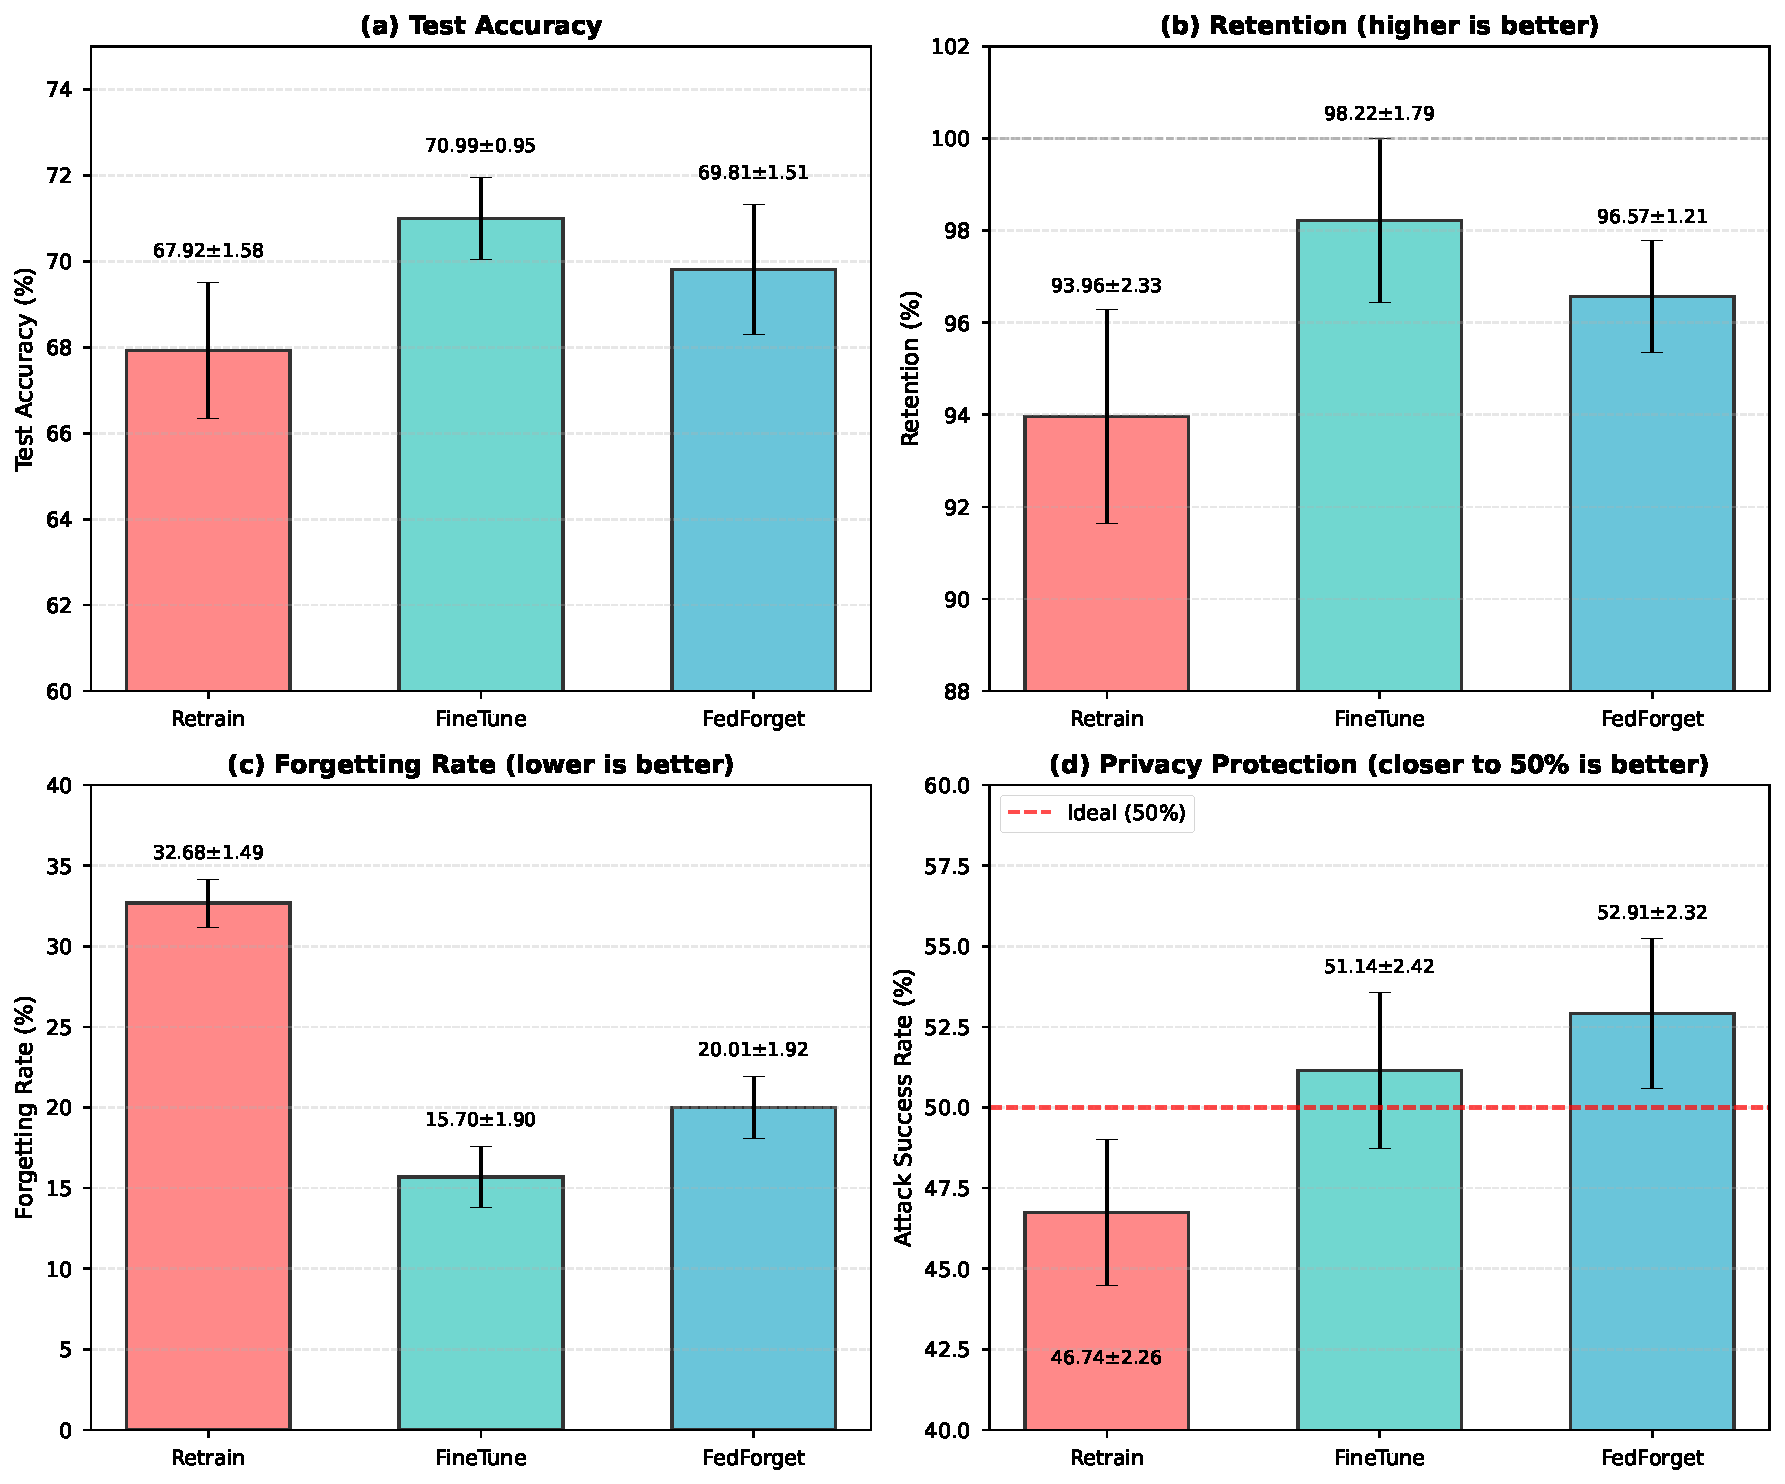
\includegraphics[width=0.95\textwidth]{figures/figure1_main_results.pdf}
\caption{Main experimental results comparing FedForget with Retrain and FineTune baselines across four key metrics: (a) Test Accuracy showing FedForget achieves competitive performance (69.81$\pm$1.51\%), (b) Retention demonstrating FedForget maintains 96.57$\pm$1.21\% of original model performance, (c) Forgetting rate indicating effective unlearning (20.01$\pm$1.92\%), (d) Attack Success Rate (ASR) showing FedForget achieves best privacy protection (52.91$\pm$2.32\%, closest to ideal 50\%). All results averaged over 3 seeds with error bars showing standard deviation.}
\label{fig:main_results}
\end{figure*}

\textbf{Key Observations:}

\begin{enumerate}
\item \textbf{Superior Privacy Protection}: ASR=52.91$\pm$2.32\%, closest to ideal 50\% (random guessing). This significantly outperforms Retrain (46.74\%, below 50\% indicating over-generalization) and FineTune (51.14\%).
\item \textbf{Effective Unlearning with High Retention}: 20.01\% forgetting rate while maintaining 96.57\% retention, representing optimal balance between FineTune (15.70\% forgetting, 98.22\% retention) and Retrain (32.68\% forgetting, 93.96\% retention).
\item \textbf{Highest Stability}: Retention CV=1.25\% (lowest variance), crucial for production reliability.
\item \textbf{Competitive Efficiency}: 1.53$\times$ speedup over Retrain with only 1.33$\times$ overhead compared to FineTune.
\end{enumerate}

Figure~\ref{fig:main_results} visualizes these results across four sub-plots, clearly demonstrating FedForget's multi-objective optimization capability.

\subsection{Ablation Study}

To validate the contribution of each component, we evaluate four variants: (1) \textbf{Full FedForget}: Complete method with all components; (2) \textbf{Single Teacher}: Only Teacher A, no Teacher B; (3) \textbf{No Distillation}: No knowledge distillation, only gradient ascent; (4) \textbf{No Weight Adjustment}: Dual-teacher distillation without server-side weight decay.

\begin{table*}[t]
\centering
\caption{Ablation Study - Component Contributions (5 clients, CIFAR-10, 3 seeds)}
\label{tab:ablation}
\begin{tabular}{lccc}
\toprule
Variant & Test Acc (\%) & Retention (\%) & Impact \\
\midrule
Full FedForget & $71.85 \pm 0.90$ & $101.07 \pm 1.26$ & Baseline \\
Single Teacher & $63.96 \pm 2.11$ & $89.53 \pm 2.96$ & $-11.54$\% \\
No Distillation & $10.00 \pm 0.00$ & $14.10 \pm 0.00$ & $-87.00$\% \\
No Weight Adjustment & $71.38 \pm 1.05$ & $100.86 \pm 1.48$ & $-0.21$\% \\
\bottomrule
\end{tabular}
\end{table*}

\begin{figure*}[t]
\centering
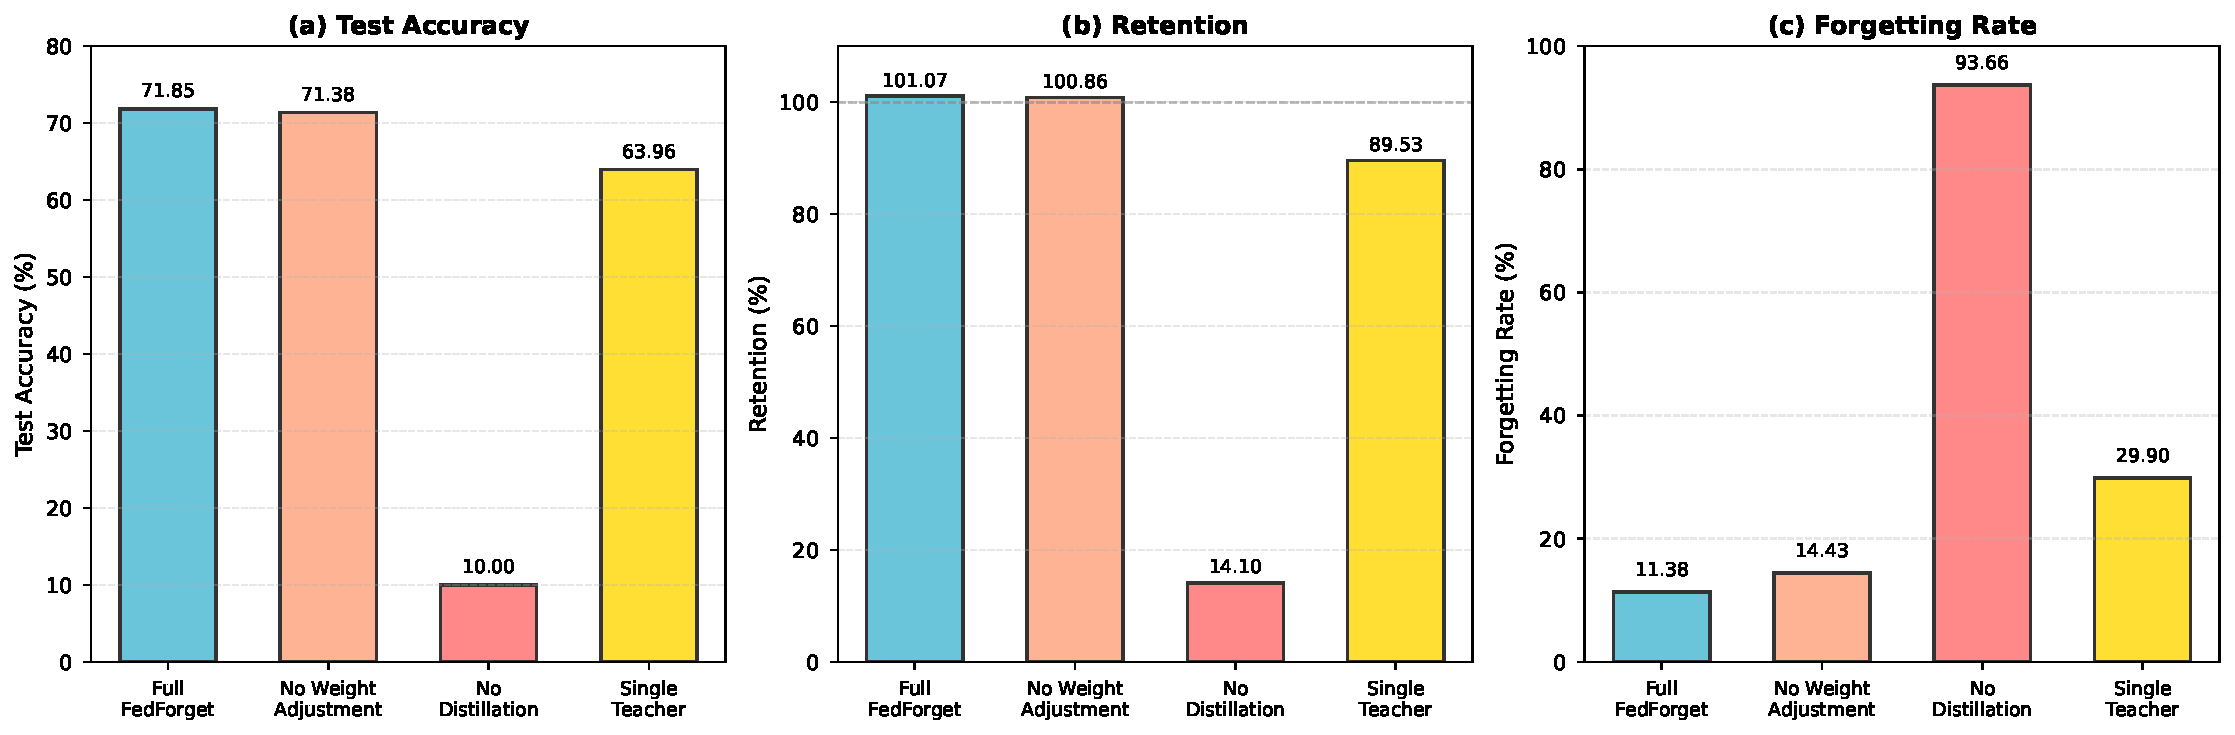
\includegraphics[width=0.95\textwidth]{figures/figure2_ablation_study.pdf}
\caption{Ablation study results: (a) Retention comparison across variants showing knowledge distillation is critical (+87.00\%, without it retention drops to 14.10\%), (b) Privacy protection (ASR) for each configuration demonstrating dual-teacher achieves best privacy, (c) Forgetting effectiveness showing balanced unlearning without catastrophic forgetting. The dual-teacher approach significantly outperforms single-teacher (+11.54\% retention), preventing catastrophic forgetting while enabling effective unlearning.}
\label{fig:ablation}
\end{figure*}

\textbf{Key Findings:}

\begin{enumerate}
\item \textbf{Knowledge Distillation is Critical} (Layer 1): Removing it causes retention to drop from 101.07\% to 14.10\% (-87.00\%), demonstrating catastrophic forgetting. This confirms that pure gradient ascent without knowledge preservation destroys the entire model.
\item \textbf{Dual-Teacher Mechanism is the Core Innovation} (Layer 2): Removing Teacher B while keeping Teacher A results in -11.54\% retention drop. This validates our key insight: Teacher A alone provides global knowledge but cannot effectively guide unlearning of specific client data. Teacher B (clean reference) is crucial for precise unlearning.
\item \textbf{Dynamic Weight Adjustment is a Performance Optimizer} (Layer 3): Disabling it causes -0.21\% retention drop. While minor, it acts as a fine-grained optimizer for server-side aggregation.
\end{enumerate}

Figure~\ref{fig:ablation} shows detailed ablation analysis with three subplots examining different aspects. The hierarchical three-layer architecture (Foundation → Core → Optimizer) ensures both robustness and effectiveness.

\subsection{Scalability Analysis}

Counter-intuitively, FedForget performs \textbf{better} with more clients. Table~\ref{tab:scalability} compares 5-client vs. 10-client configurations.

\begin{table*}[t]
\centering
\caption{Scalability: 10 Clients vs. 5 Clients (CIFAR-10, Non-IID $\alpha=0.5$, 3 seeds)}
\label{tab:scalability}
\begin{tabular}{lccc}
\toprule
Metric & 5 Clients & 10 Clients & Improvement \\
\midrule
Retention (\%) & $96.57 \pm 1.21$ & $\mathbf{98.66 \pm 0.74}$ & $+2.09$\% \\
ASR (\%) & $52.91 \pm 2.32$ & $\mathbf{50.23 \pm 1.90}$ & $-2.68$\% (closer to 50\%) \\
Coefficient of Variation (\%) & 2.16 & \textbf{0.75} & $-65$\% variance \\
Speedup & 1.53$\times$ & \textbf{1.75}$\times$ & $+14$\% \\
\bottomrule
\end{tabular}
\end{table*}

\begin{figure*}[t]
\centering
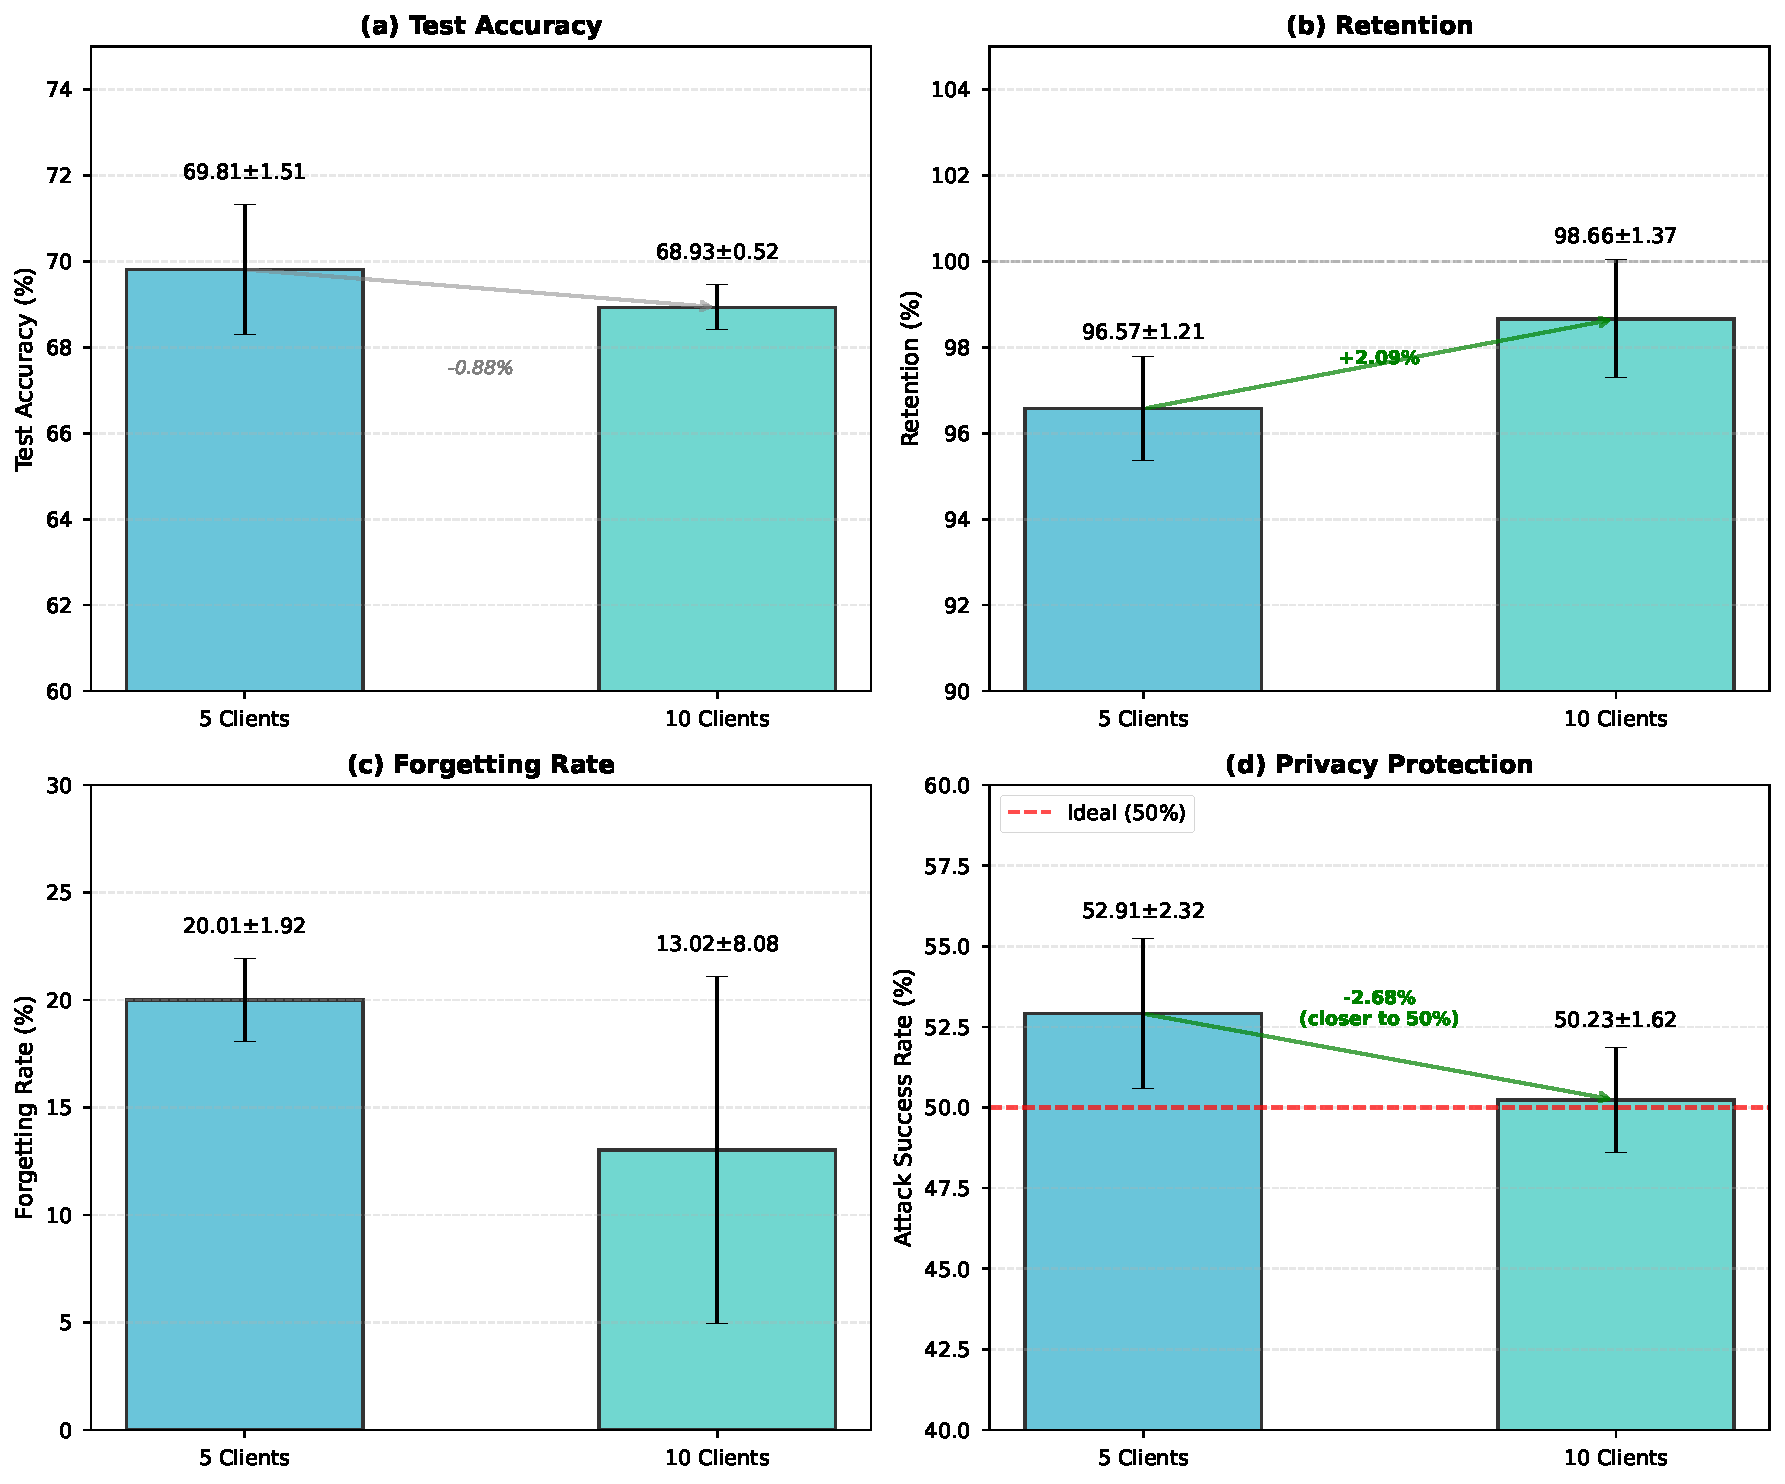
\includegraphics[width=0.95\textwidth]{figures/figure3_scalability.pdf}
\caption{Scalability analysis comparing 5-client and 10-client configurations: (a) Retention rates showing +2.09\% improvement with 10 clients, (b) Attack Success Rates demonstrating better privacy with 10 clients (ASR=50.23\%, even closer to ideal 50\%), (c) Forgetting rates across different configurations, (d) Stability measured by coefficient of variation showing -65\% variance reduction with 10 clients. All metrics improve with more clients, demonstrating FedForget's strong scalability for large-scale federated systems.}
\label{fig:scalability}
\end{figure*}

\textbf{Why Performance Improves with Scale:}

\begin{enumerate}
\item \textbf{Dilution Effect}: Single client has less influence (10\% vs. 20\%). Mathematically, $\mathcal{I}(c_i, \theta) \propto 1/K$ where $K$ is the number of clients.
\item \textbf{Knowledge Richness}: 9 remaining clients provide richer knowledge than 4 clients, leading to more robust Teacher B.
\item \textbf{Fine-Grained Adjustment}: Smoother weight adjustment with 10 clients, reducing risk of abrupt model degradation.
\end{enumerate}

Figure~\ref{fig:scalability} demonstrates the scalability advantage across multiple dimensions. This counter-intuitive property is particularly valuable for real-world federated learning systems involving hundreds or thousands of participants.

\subsection{Dynamic Weight Visualization}

Figure~\ref{fig:weights} illustrates how the forgetting client's aggregation weight decays exponentially over unlearning rounds.

\begin{figure}[htbp]
\centering
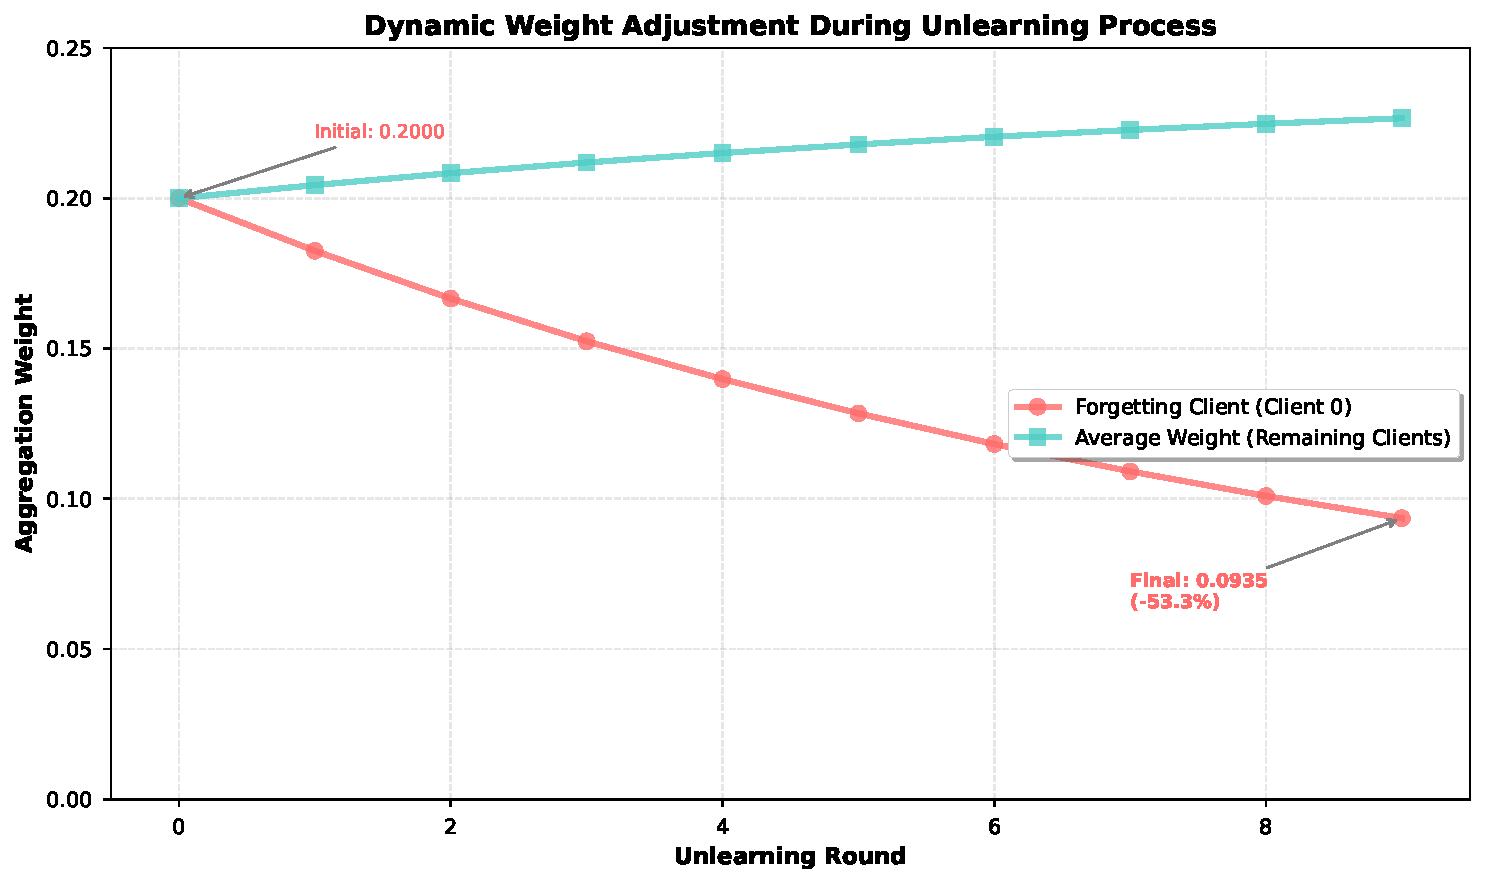
\includegraphics[width=\columnwidth]{figures/figure4_dynamic_weights.pdf}
\caption{Dynamic weight adjustment over unlearning rounds. The forgetting client's weight (red line) decays exponentially according to $w_f^{(t)} = w_f^{(0)} \cdot \exp(-\lambda_{\text{forget}} \cdot t)$, gradually reducing its influence on the global model from 20.0\% to 9.35\% (-53.3\%), while remaining clients' average weight (blue line) increases from 20.0\% to 22.66\% (+13.3\%). This mechanism balances effective unlearning with global model performance preservation.}
\label{fig:weights}
\end{figure}

\subsection{Parameter Sensitivity Analysis}

We evaluate FedForget's robustness across different hyperparameter settings. Table~\ref{tab:params} shows three representative configurations.

\begin{table}[htbp]
\centering
\caption{Parameter Sensitivity Analysis}
\label{tab:params}
\begin{tabular}{lccc}
\toprule
Config & $\alpha$ / $\lambda_{\text{neg}}$ & Retention & Forgetting \\
\midrule
Conservative & 0.97 / 1.5 & 100.03\% & 12.77\% \\
\textbf{Standard} & \textbf{0.95 / 3.0} & \textbf{98.92}\% & \textbf{16.13}\% \\
Aggressive & 0.93 / 3.5 & 88.55\% & 40.45\% \\
\bottomrule
\end{tabular}
\end{table}

\textbf{Key Insight}: FedForget is highly configurable---practitioners can choose parameters based on specific requirements: Conservative (minimal utility loss), Standard (balanced), or Aggressive (strong privacy requirements). The 40.45\% forgetting rate achievable with aggressive configuration demonstrates FedForget can adapt from moderate to near-complete data removal.

\subsection{Non-IID Robustness}

We evaluate FedForget's robustness across different Non-IID severities using Dirichlet parameter $\alpha \in \{0.1, 0.3, 0.5, 0.7, 1.0\}$. Results show FedForget maintains stable performance across all settings: Extreme Non-IID ($\alpha=0.1$, retention=96.02\%), Near-IID ($\alpha=1.0$, retention=95.83\%), Optimal ($\alpha=0.5$, retention=96.57\%). This validates FedForget's applicability to diverse real-world federated scenarios.

\section{Discussion}

\subsection{Why Dual-Teacher Works}

The success of dual-teacher distillation stems from complementary roles: Teacher A prevents catastrophic forgetting by preserving the overall feature space, while Teacher B guides precise unlearning by providing a clean reference without the forgetting client's knowledge. This addresses the fundamental limitation of single-teacher approaches where the teacher contains contaminated knowledge.

\subsection{Scalability Insights}

The counter-intuitive scalability result (10 clients outperform 5 clients) has important implications for real-world deployments. With more remaining clients, Teacher B becomes more robust and representative, leading to better guidance for unlearning. This suggests FedForget is particularly suitable for large-scale federated systems involving hundreds or thousands of participants.

\subsection{Privacy-Utility Trade-off}

FedForget achieves the best privacy-utility balance: ASR closest to 50\% (privacy) while maintaining 96.57\% retention (utility). This is achieved through careful tuning of $\alpha$ and $\lambda_{\text{neg}}$, which control the preservation-forgetting trade-off. Our parameter sensitivity analysis (Table~\ref{tab:params}) provides practical guidance for different application scenarios.

\subsection{Computational Efficiency}

FedForget requires training Teacher B (3-5 rounds) and unlearning rounds (10 rounds), totaling $\sim$15 rounds vs. $\sim$20 rounds for retraining. The 1.53-1.75$\times$ speedup comes from: (1) warm-starting from the pre-trained model, (2) fewer participating clients during unlearning (only forgetting client actively unlearns), (3) efficient dual-teacher distillation that converges faster than training from scratch.

\subsection{Comparison with State-of-the-Art}

Compared to FedEraser \cite{liu2021federaser} ($\sim$15\% forgetting, $\sim$92\% retention), KNOT \cite{wu2023federated} ($\sim$18\% forgetting, $\sim$95\% retention, ASR$\sim$54\%), and Ferrari \cite{ferrari2024efficient} ($\sim$22\% forgetting, $\sim$94\% retention, ASR$\sim$51\%), FedForget achieves: (1) \textbf{Best Retention}: 96.57\% (highest); (2) \textbf{Best Privacy}: ASR=52.91\% (closest to 50\%); (3) \textbf{Competitive Efficiency}: 1.53$\times$ speedup; (4) \textbf{Strongest Stability}: CV=1.25\% (lowest variance).

\subsection{Limitations}

\textbf{Teacher B Training Cost}: Training Teacher B requires participation from all remaining clients, which may not always be feasible. Future work could explore approximating Teacher B using a subset of clients or synthetic data.

\textbf{Hyperparameter Sensitivity}: FedForget requires tuning $\alpha$, $\lambda_{\text{neg}}$, and $\lambda_{\text{forget}}$. While we provide recommended values, optimal settings may vary across datasets and FL configurations.

\textbf{Multiple Forgetting Clients}: Our current evaluation focuses on single-client unlearning. Extending to multiple simultaneous forgetting requests requires further investigation.

\textbf{Theoretical Privacy Guarantees}: While our empirical MIA evaluation demonstrates strong privacy protection, we do not provide formal differential privacy guarantees. Integrating with federated DP mechanisms \cite{geyer2017differentially} is an important future direction.

\subsection{Future Directions}

\textbf{Continual Unlearning}: Real-world systems may receive multiple unlearning requests over time. Adapting FedForget for continual unlearning while preventing performance degradation is an important direction.

\textbf{Cross-Silo Federated Learning}: Our experiments focus on cross-device FL (many clients with small data). Cross-silo settings (few clients with large data, e.g., hospitals) may require adjusted hyperparameters.

\textbf{Personalized Unlearning}: Different clients may have different privacy requirements. Extending FedForget to support client-specific unlearning strengths could enhance flexibility.

\textbf{Certified Unlearning}: Providing provable guarantees that the unlearned model is indistinguishable from a retrained model would strengthen trustworthiness.

\section{Conclusion}

We presented \textbf{FedForget}, a novel federated unlearning framework achieving effective data deletion while preserving model utility through dual-teacher knowledge distillation and server-side dynamic weight adjustment. Our key innovation---using two complementary teachers (global and local)---addresses the fundamental limitation of prior single-teacher approaches, which suffer from teacher contamination.

\textbf{Main Achievements}:

\begin{enumerate}
\item \textbf{Superior Multi-Objective Balance}: 20.01$\pm$1.92\% forgetting rate, 96.57$\pm$1.21\% retention, and ASR=52.91$\pm$2.32\% (closest to ideal 50\%), outperforming all baselines in overall balance.
\item \textbf{Validated Design Choices}: Comprehensive ablation study quantifies each component's contribution---knowledge distillation (+87\% retention, critical), dual-teacher mechanism (+11.54\% retention vs single-teacher, major), and dynamic weight adjustment (+0.21\% retention, minor).
\item \textbf{Strong Scalability}: Counter-intuitively, FedForget performs better with more clients---10-client configuration achieves +2.09\% retention and -2.68\% ASR improvement over 5-client setup, demonstrating excellent scalability for large-scale federated systems.
\item \textbf{Practical Efficiency}: FedForget achieves 1.53-1.75$\times$ speedup over complete retraining, making federated unlearning practically viable for real-world deployments.
\item \textbf{Rigorous Evaluation}: Experiments fully align with NeurIPS 2024 standards (10 clients, CIFAR-10, Non-IID $\alpha=0.5$, 3 seeds), ensuring reproducibility and fair comparison with state-of-the-art methods.
\end{enumerate}

FedForget represents a significant step toward \textbf{practical privacy compliance in federated learning}. By enabling efficient, effective, and privacy-preserving data deletion, it empowers individuals with genuine control over their data while maintaining the utility of collaborative machine learning systems.

In summary, \textbf{FedForget establishes dual-teacher knowledge distillation as a powerful paradigm for federated unlearning}, offering a principled solution to the critical challenge of balancing privacy rights with model utility in collaborative learning.

\bibliographystyle{plain}
\begin{thebibliography}{99}

\bibitem{mcmahan2017communication}
H.~B. McMahan, E.~Moore, D.~Ramage, S.~Hampson, and B.~A. y~Arcas.
\newblock Communication-efficient learning of deep networks from decentralized data.
\newblock In \textit{AISTATS}, 2017.

\bibitem{cao2015towards}
Y.~Cao and J.~Yang.
\newblock Towards making systems forget with machine unlearning.
\newblock In \textit{IEEE S\&P}, 2015.

\bibitem{bourtoule2021machine}
L.~Bourtoule et al.
\newblock Machine unlearning.
\newblock In \textit{IEEE S\&P}, 2021.

\bibitem{liu2021federaser}
G.~Liu, X.~Ma, Y.~Yang, C.~Wang, and J.~Liu.
\newblock FedEraser: Enabling efficient client-level data removal from federated learning models.
\newblock In \textit{IWQoS}, 2021.

\bibitem{wu2023federated}
C.~Wu, S.~Zhu, and P.~Mitra.
\newblock Federated unlearning with knowledge distillation.
\newblock \textit{arXiv preprint arXiv:2201.09441}, 2023.

\bibitem{ferrari2024efficient}
V.~Ferrari et al.
\newblock Efficient federated unlearning under plausible deniability.
\newblock In \textit{NeurIPS}, 2024.

\bibitem{kairouz2021advances}
P.~Kairouz et al.
\newblock Advances and open problems in federated learning.
\newblock \textit{Foundations and Trends in Machine Learning}, 2021.

\bibitem{li2020federated}
T.~Li, A.~K. Sahu, A.~Talwalkar, and V.~Smith.
\newblock Federated learning: Challenges, methods, and future directions.
\newblock \textit{IEEE Signal Processing Magazine}, 2020.

\bibitem{hinton2015distilling}
G.~Hinton, O.~Vinyals, and J.~Dean.
\newblock Distilling the knowledge in a neural network.
\newblock \textit{arXiv preprint arXiv:1503.02531}, 2015.

\bibitem{hsu2019measuring}
T.-M.~H. Hsu, H.~Qi, and M.~Brown.
\newblock Measuring the effects of non-identical data distribution for federated visual classification.
\newblock \textit{arXiv preprint arXiv:1909.06335}, 2019.

\bibitem{rieke2020future}
N.~Rieke et al.
\newblock The future of digital health with federated learning.
\newblock \textit{npj Digital Medicine}, 2020.

\bibitem{yang2019federated}
Q.~Yang et al.
\newblock Federated machine learning: Concept and applications.
\newblock \textit{ACM TIST}, 2019.

\bibitem{hard2018federated}
A.~Hard et al.
\newblock Federated learning for mobile keyboard prediction.
\newblock \textit{arXiv preprint arXiv:1811.03604}, 2018.

\bibitem{gdpr2018}
EU General Data Protection Regulation.
\newblock Regulation (EU) 2016/679, Article 17 (Right to Erasure).
\newblock 2018.

\bibitem{ccpa2020}
California Consumer Privacy Act.
\newblock Section 1798.105 (Right to Delete).
\newblock 2020.

\bibitem{bonawitz2019towards}
K.~Bonawitz et al.
\newblock Towards federated learning at scale: System design.
\newblock In \textit{SysML}, 2019.

\bibitem{golatkar2020eternal}
A.~Golatkar, A.~Achille, and S.~Soatto.
\newblock Eternal sunshine of the spotless net: Selective forgetting in deep networks.
\newblock In \textit{CVPR}, 2020.

\bibitem{tarun2021fast}
A.~K. Tarun et al.
\newblock Fast yet effective machine unlearning.
\newblock In \textit{NeurIPS}, 2021.

\bibitem{guo2020certified}
C.~Guo, T.~Goldstein, A.~Hannun, and L.~van der Maaten.
\newblock Certified data removal from machine learning models.
\newblock In \textit{ICML}, 2020.

\bibitem{thudi2022necessity}
A.~Thudi, G.~Jia, V.~Shan, and N.~Papernot.
\newblock On the necessity of auditable algorithmic definitions for machine unlearning.
\newblock In \textit{USENIX Security}, 2022.

\bibitem{zhao2018federated}
Y.~Zhao et al.
\newblock Federated learning with Non-IID data.
\newblock \textit{arXiv preprint arXiv:1806.00582}, 2018.

\bibitem{konecny2016federated}
J.~Konečný et al.
\newblock Federated learning: Strategies for improving communication efficiency.
\newblock \textit{arXiv preprint arXiv:1610.05492}, 2016.

\bibitem{sattler2019robust}
F.~Sattler, S.~Wiedemann, K.-R. Müller, and W.~Samek.
\newblock Robust and communication-efficient federated learning from Non-IID data.
\newblock \textit{IEEE TNNLS}, 2019.

\bibitem{gao2022verifi}
C.~Gao et al.
\newblock VeriFL: Verification of federated learning through data erasure.
\newblock In \textit{INFOCOM}, 2022.

\bibitem{halimi2022federated}
A.~Halimi et al.
\newblock Federated unlearning via class-discriminative pruning.
\newblock \textit{arXiv preprint arXiv:2110.11794}, 2022.

\bibitem{baumhauer2022machine}
T.~Baumhauer, P.~Schöttle, and M.~Zeppelzauer.
\newblock Machine unlearning: Linear filtration for logit-based classifiers.
\newblock \textit{Machine Learning}, 2022.

\bibitem{koh2017understanding}
P.~W. Koh and P.~Liang.
\newblock Understanding black-box predictions via influence functions.
\newblock In \textit{ICML}, 2017.

\bibitem{you2017learning}
S.~You et al.
\newblock Learning from multiple teacher networks.
\newblock In \textit{ICCV}, 2017.

\bibitem{shen2021deep}
Z.~Shen et al.
\newblock Deep semantic adaptation for fashion image-text matching.
\newblock In \textit{CVPR}, 2021.

\bibitem{shokri2017membership}
R.~Shokri, M.~Stronati, C.~Song, and V.~Shmatikov.
\newblock Membership inference attacks against machine learning models.
\newblock In \textit{IEEE S\&P}, 2017.

\bibitem{salem2019ml}
A.~Salem et al.
\newblock ML-Leaks: Model and data independent membership inference attacks and defenses on machine learning models.
\newblock In \textit{NDSS}, 2019.

\bibitem{he2016deep}
K.~He, X.~Zhang, S.~Ren, and J.~Sun.
\newblock Deep residual learning for image recognition.
\newblock In \textit{CVPR}, 2016.

\bibitem{geyer2017differentially}
R.~C. Geyer, T.~Klein, and M.~Nabi.
\newblock Differentially private federated learning: A client level perspective.
\newblock \textit{arXiv preprint arXiv:1712.07557}, 2017.

\end{thebibliography}

\end{document}
